\section{MC for \MITL\ over timelines}\label{sec:modelcheckingTimelines}

In this section we deal with the ultimate goal of the present chapter:
as mentioned, we want to model check systems specified in terms of timelines. More precisely, 
a system is described as a set of state variables along with a set of synchronization rules over them (a TP domain) $P=(SV,R)$.
As mentioned in the introduction, the property specification language we will be assuming is the logic \MITL.
%%
%Henceforth, $\Prop$ denotes a set of proposition letters.

We first recall the encoding of multi-timelines already adopted in Section~\ref{sec:Reduction}, 
over which we interpret \MITL,
that exploits 
the set $\Prop$ of proposition letters
\[
\Prop = \bigcup_{x\in SV}\Main_x \cup \Deriv ,
\] 
where in particular
\[
\Main_x = ((\{\Beg_x \}\cup V_x) \times V_x)   \cup   (V_x \times \{\End_x\}).
\]
The tags $\Beg_x$ and $\End_x$ mark the beginning and the end of a timeline for $x$, and a pair $(v,v')\in \Main_x$ represents a 
transition of the value taken by $x$ from $v$ to $v'$ (a token for $x$ with value $v'$ follows a token with value $v$).
The already introduced formula 
\[
\psi(\start,v)= (\Beg_x,v)\vee \displaystyle{\bigvee_{u\in V_x}}(u,v),
\]
states that a start-event for a token for $x$ with value $v$ occurs at the current time.
Finally, $\EqTime(\theta) = \theta \vee [\neg p_> \StrictUntil_{\geq 0}(\neg p_> \wedge \theta)]$, where $p_>\in\Deriv$, is satisfied
by an encoding of a multi-timeline at the current time if $\theta$ eventually holds at a position whose timestamp coincides with the current one.

Before formalizing the \emph{MC problem for \MITL\ formulas over timelines}, we want to start with an easy example of a system whose components are described by timelines, over which we check some properties encoded by \MITL\ formulas.

\begin{figure}[p]
    \centering
    \resizebox{!}{0.9\textheight}{\rotatebox{90}{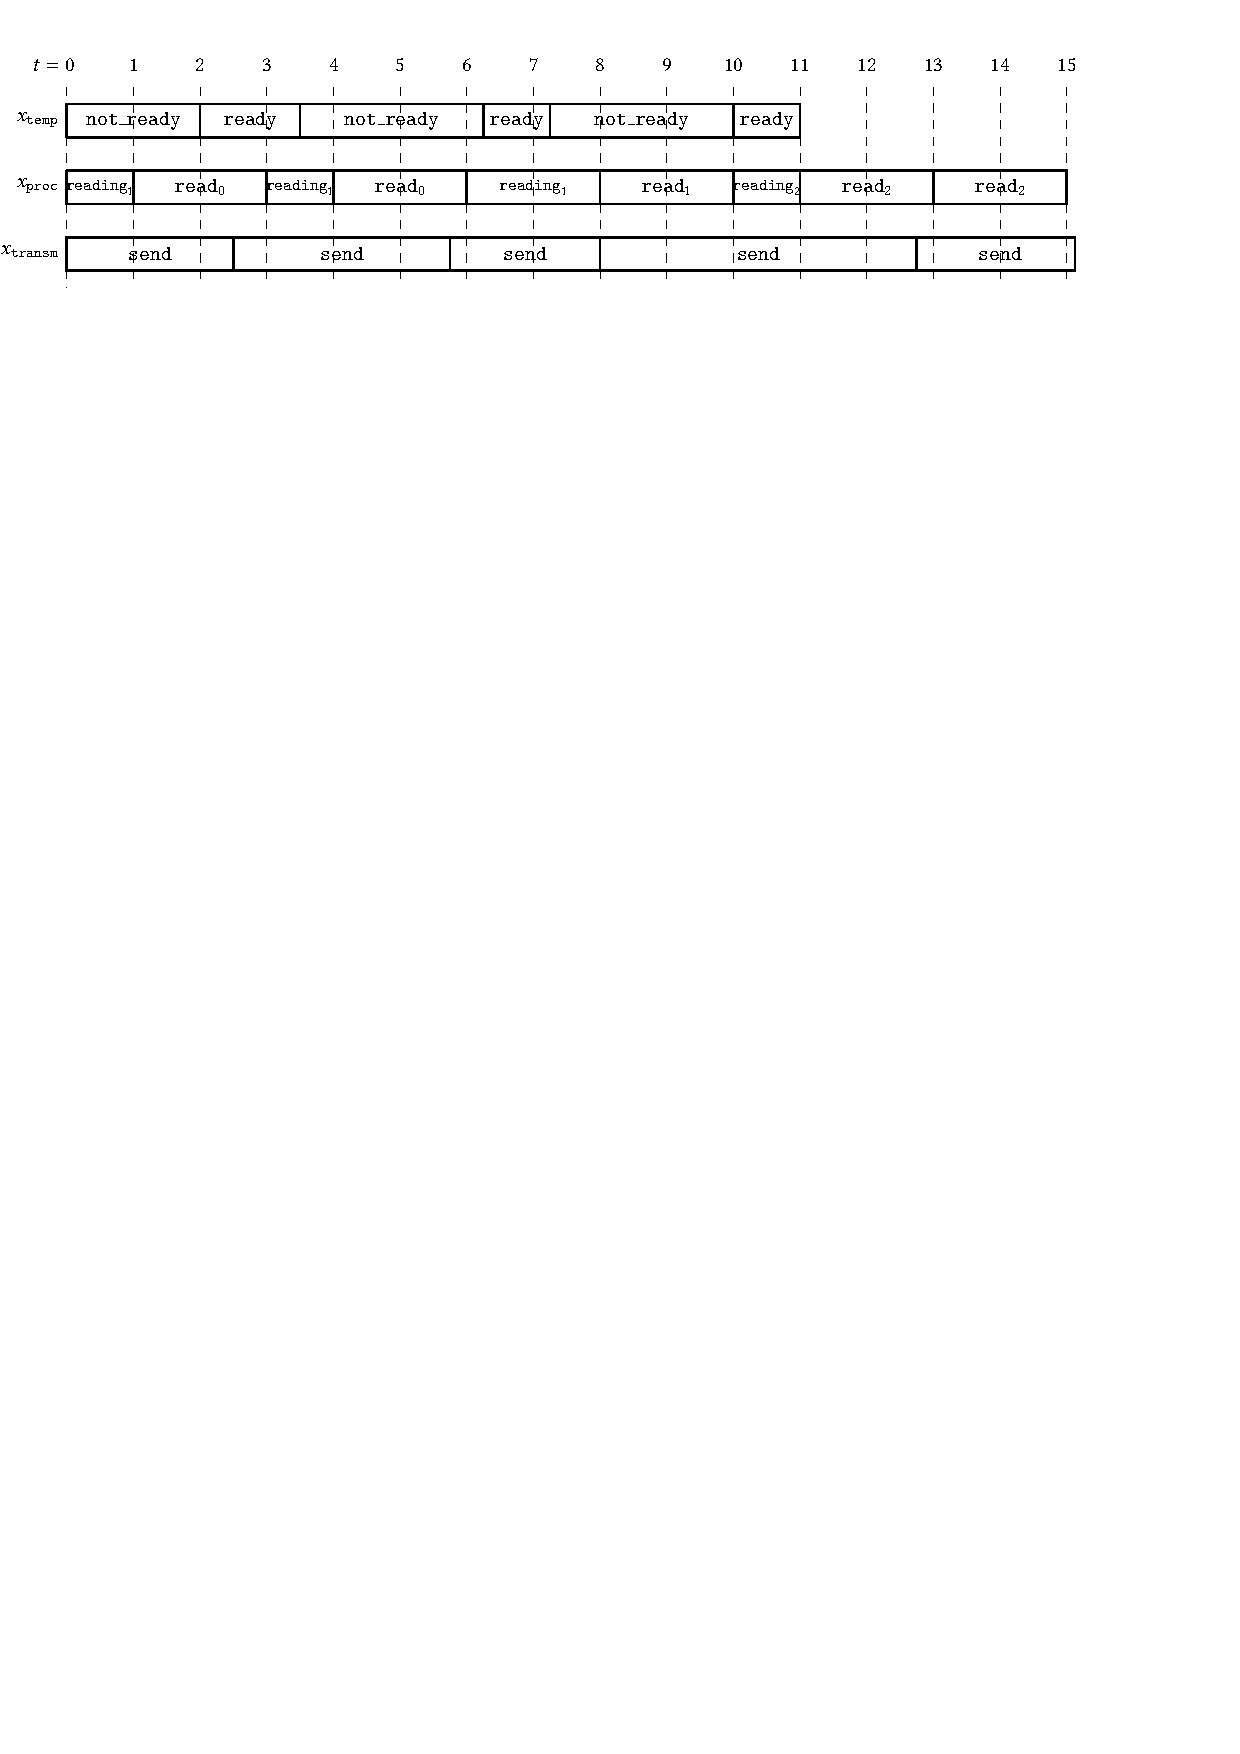
\includegraphics{Chaps/Timelines/exPlan.pdf}}}
    \caption{Example of computation for the defined system}
    \label{fig:explan}
\end{figure}

\begin{example}
Let us consider the following system, consisting of a \emph{temperature sensor}, a \emph{processing unit}, and a \emph{data transmission unit}.
These components are modelled by three state variables, $x_\mathtt{temp}=(V_\mathtt{temp},T_\mathtt{temp},D_\mathtt{temp})$, $x_\mathtt{proc}=(V_\mathtt{proc},T_\mathtt{proc},D_\mathtt{proc})$ and $x_\mathtt{transm}=(V_\mathtt{transm},T_\mathtt{transm},D_\mathtt{transm})$, where
\begin{itemize}
    \item $V_\mathtt{temp}=\{\mathtt{ready}, \mathtt{not\_ready}\}$, \\
    $T_\mathtt{temp}(\mathtt{ready})=\{\mathtt{not\_ready}\}$, $T_\mathtt{temp}(\mathtt{not\_ready})=\{\mathtt{ready}\}$, \\ $D_\mathtt{temp}(\mathtt{ready})=[1,2]$, $D_\mathtt{temp}(\mathtt{not\_ready})=[2,3]$;
    \item $V_\mathtt{proc}=\{\mathtt{reading}_1,\mathtt{reading}_2,\mathtt{read}_0,\mathtt{read}_1,\mathtt{read}_2\}$, \\
    $T_\mathtt{proc}(\mathtt{reading}_1)=\{\mathtt{read}_0,\mathtt{read}_1\}$,
    $T_\mathtt{proc}(\mathtt{reading}_2)=\{\mathtt{read}_1,\allowbreak \mathtt{read}_2\}$,
    $T_\mathtt{proc}(\mathtt{read}_0)=\{\mathtt{reading}_1\}$, $T_\mathtt{proc}(\mathtt{read}_1)=\{\mathtt{reading}_2\}$,
    $T_\mathtt{proc}(\mathtt{read}_2)=\{\mathtt{read}_2\}$, \\
    $D_\mathtt{proc}(\mathtt{reading}_1)=D_\mathtt{proc}(\mathtt{reading}_2)=[1,2]$, $D_\mathtt{proc}(\mathtt{read}_0)=D_\mathtt{proc}(\mathtt{read}_1)=D_\mathtt{proc}(\mathtt{read}_2)=[2,3]$;
    \item $V_\mathtt{transm}=\{\mathtt{send}\}$,\\
    $T_\mathtt{transm}(\mathtt{send})=\{\mathtt{send}\}$,\\
    $D_\mathtt{transm}(\mathtt{send})=[2,5]$.
\end{itemize}

The temperature sensor alternates between the two states $\mathtt{ready}$ and $\mathtt{not\_ready}$. In the former, it senses the temperature of the environment and \emph{possibly} sends the temperature value to the processing unit.
The purpose of the processing unit is receiving \emph{two} temperature samples from the sensor, and sending the average value to the data transmission unit. While in state $\mathtt{read}_i$, for $i=0,1,2$, it has read $i$ samples. While in $\mathtt{reading}_j$, for $j=1,2$, it is attempting to read the $j$-th sample. A reading is possible only if the sensor and the processing unit are synchronized: a time interval (token) with value $\mathtt{reading}_j$ has to \emph{contain} (Allen relation, see Table~\ref{allen}) a token $\mathtt{ready}$. 
Analogously, the processing unit can send data to the transmitter only if a token with value $\mathtt{send}$ contains one with value $\mathtt{read}_2$.

The sensor starts in state $\mathtt{not\_ready}$. This is specified by the trigger-less rule $\true\to\exists o[x_\mathtt{temp} = \mathtt{not\_ready}]. o\leq^\start_{[0,0]} 0$. The processing unit starts in state $\mathtt{reading}_1$: $\true\to\exists o[x_\mathtt{proc} = \mathtt{reading}_1]. o\leq^\start_{[0,0]} 0$.
(Recall that trigger-less rules may also contain singular intervals at no extra computational cost.)
The goal of the system is encoded by the rule
$\true\to \exists o_1 [x_\mathtt{proc} = \mathtt{read}_2] \exists o_2 [x_\mathtt{transm} = \mathtt{send}]. (o_2 \leq^{\start,\start}_{\mathopen[0,+\infty\mathclose[} o_1 \wedge o_1 \leq^{\Ending,\Ending}_{\mathopen[0,+\infty\mathclose[} o_2)$.

Let us now encode the fact that the sensor and the processing unit must be synchronized for the latter to receive a temperature sample.
We assume the next simple trigger rule to be \emph{interpreted under the future semantics}.
\begin{multline}\label{eq:sync}
o[x_\mathtt{proc} = \mathtt{reading}_1] \to (\exists o_1[x_\mathtt{proc} = \mathtt{read}_0]. o \leq_{[0,1]}^{\Ending,\start} o_1) \vee\\ (\exists o_2[x_\mathtt{proc} = \mathtt{read}_1] \exists o_3[x_\mathtt{temp} = \mathtt{ready}]. o \leq_{[0,1]}^{\Ending,\start} o_2\wedge o_3\leq_{\mathopen[0,+\infty\mathclose[}^{\Ending,\Ending} o).
\end{multline}
Let us observe that, due to the future semantics, the token (referenced by the name) $o$ starts no later than $o_3$: this with the interval atom \mbox{$o_3\leq_{\mathopen[0,+\infty\mathclose[}^{\Ending,\Ending} o$} force the \emph{contains} Allen relation between $o$ and $o_3$.
An analogous rule can be written for the second temperature sample (where $x_\mathtt{proc}=\mathtt{reading}_2$).

In Figure~\ref{fig:explan} we show an example of plan/computation for the system described by $P=(\{x_\mathtt{temp},x_\mathtt{proc},x_\mathtt{transm}\},R)$.

Let us now specify some properties in \MITL\ (more precisely, $\MITLR$) to check on the system model. The idea is that such properties must hold true over \emph{all possible computations (plans)} of the described system, in order for the MC problem to be satisfied.

\begin{itemize}
    \item $\Always_{<2}\;\neg \psi(\start,\mathtt{ready})$. This property holds true in any system computation, as the sensor does not ever get ready by 2 seconds;
    \item $\Eventually_{\leq 8}\; \psi(\start,\mathtt{read}_1)$. This property is not true in all computations (but it is, e.g., in the one of Figure~\ref{fig:explan}), because the sensor and the processing unit may synchronize for the first time after 8 seconds;
    \item $\Eventually_{\geq 0}\big(\psi(\start,\mathtt{ready}) \wedge (\true\until_{>0}\;\psi(\start,\mathtt{ready}))\big)$. This property holds true in any system computation, since the system guarantees, after some time, to eventually send the data via the transmitter. In order for this to happen, the sensor must become ready (at least) twice.
    \item $\Always_{\geq 0} \big(\psi(\start,\mathtt{read}_1) \to \Eventually_{\leq 3}\; \psi(\start,\mathtt{read}_2)\big)$. % \!\wedge\! (\EqTime(\psi(\start,\mathtt{send}))\!\vee\! \Past_\mathtt{send}^{\start}) \big)$. 
    This property is not true in all computations as the processing unit, after reading the first sample, may not be able to read the second one by 3 time units (e.g., when the transmitter and the processing unit do not synchronize as soon as possible).
    \item {\small $\Always_{\geq 0} \big(\psi(\start,\mathtt{reading}_1) \!\wedge\! (\EqTime(\psi(\start,\mathtt{ready}))\!\vee\! \Past_\mathtt{ready}^{\start}) \!\to\! \Eventually_{\leq 2}\, \psi(\start,\mathtt{read}_1) \big)$}. 
    We recall that the proposition letter $\Past_\mathtt{ready}^{\start}$ is true at the time it is interpreted if there is a past token for $x_\mathtt{temp}$ with value $\mathtt{ready}$ starting at the same timestamp. 
%
    The formula considers a situation where a token with value $\mathtt{reading}_1$ starts together with a token $\mathtt{ready}$. %Since the minum duration of is less than the minimum of, this is a synch. However,
    The property expressed by the formula is not true in general, as either 
    $(i)$~the token $\mathtt{reading}_1$ may not contain the token $\mathtt{ready}$, hence $x_\mathtt{proc}$ will not move to the state $\mathtt{read}_1$ by 2 time units, or
    $(ii)$~the token $\mathtt{reading}_1$ is followed by a token $\mathtt{read}_0$. As for the latter case,
    the system description rule (\ref{eq:sync}) states that if there is a transition from state $\mathtt{reading}_1$ to $\mathtt{read}_1$, then the processing unit and the sensors must have synchronized. However, the converse implication need not hold: the two component may fail to communicate anyway (the processing unit remaining in $\mathtt{read}_0$).
\end{itemize}
\end{example}

Let us now formally define the MC problem for \MITL\ formulas over timelines.
As shown in the proof of Theorem~\ref{theorem:UpperBounds}, given a system model $P_\text{sys}=(SV,R)$, it is possible to build a \TA\ $\mathcal{A}_\text{sys}$ that
accepts all and only the encodings $w_\Pi$ of multi-timelines $\Pi$ of $SV$ satisfying all the rules in $R$.

\begin{definition}[Model checking]
Given a system model $P_\text{sys}=(SV,R)$ and a \MITL\ formula $\varphi$ over $\Prop$, the MC problem for \MITL\ formulas over timelines is to decide whether or not $\TLang(\mathcal{A}_\text{sys})\subseteq \TLang(\varphi)$.
\end{definition}

We recall that~\cite{Alur:1996} %, as already mentioned in the proof of Theorem~\ref{theorem:UpperBounds}, 
given a \MITL\ (resp., $\MITLR$) formula $\psi$, where $N$ is the number of distinct subformulas of $\psi$, and $K$ the largest integer constant appearing in $\psi$, we can build a \TA\ $\mathcal{A}_\psi$ accepting the models of $\psi$, with $O(2^{N\cdot K})$ (resp., $O(2^{N})$) states, $O(N\cdot K)$ (resp., $O(N)$) clocks, and maximum constant $O(K)$. Deciding its emptiness requires
space \emph{logarithmic} in the number of states of $\mathcal{A}_\psi$ and \emph{polynomial}
in the number of clocks and in the length of the encoding of $K$, hence
exponential (resp., polynomial) space.

To decide if $\TLang(\mathcal{A}_\text{sys})\subseteq \TLang(\varphi)$, we check whether $\TLang(\mathcal{A}_\text{sys})\cap \TLang(\mathcal{A}_{\neg \varphi})= \emptyset$ by making the intersection $\mathcal{A}_\wedge$ of 
$\mathcal{A}_\text{sys}$ and $\mathcal{A}_{\neg \varphi}$, and checking for emptiness of its timed language. 
The size of $\mathcal{A}_\wedge$ is polynomial in those of $\mathcal{A}_\text{sys}$ and $ \mathcal{A}_{\neg \varphi}$.
Moreover $\mathcal{A}_\text{sys}$, $\mathcal{A}_{\neg \varphi}$ and $\mathcal{A}_\wedge$ can be built on the fly, and the emptiness test can be done without explicitly constructing them as well.
The next result follows by these observations and by Theorem~\ref{theorem:UpperBounds}.

\begin{theorem}
The MC problem for \MITL\ formulas over timelines, with simple future trigger rules and non-singular intervals, is in \EXPSPACE.

The MC problem for $\MITLR$ formulas over timelines, with simple future trigger rules and intervals in $\Intv_{(0,\infty)}$, is in \Psp.
\end{theorem}

Clearly, \EXPSPACE- and \Psp-completeness of the above MC problems follow by the underlying future TP problems.